\documentclass[
  man,
  floatsintext,
  longtable,
  nolmodern,
  notxfonts,
  notimes,
  colorlinks=true,linkcolor=blue,citecolor=blue,urlcolor=blue]{apa7}

\usepackage{amsmath}
\usepackage{amssymb}




\RequirePackage{longtable}
\RequirePackage{threeparttablex}

\makeatletter
\renewcommand{\paragraph}{\@startsection{paragraph}{4}{\parindent}%
	{0\baselineskip \@plus 0.2ex \@minus 0.2ex}%
	{-.5em}%
	{\normalfont\normalsize\bfseries\typesectitle}}

\renewcommand{\subparagraph}[1]{\@startsection{subparagraph}{5}{0.5em}%
	{0\baselineskip \@plus 0.2ex \@minus 0.2ex}%
	{-\z@\relax}%
	{\normalfont\normalsize\bfseries\itshape\hspace{\parindent}{#1}\textit{\addperi}}{\relax}}
\makeatother




\usepackage{longtable, booktabs, multirow, multicol, colortbl, hhline, caption, array, float, xpatch}
\setcounter{topnumber}{2}
\setcounter{bottomnumber}{2}
\setcounter{totalnumber}{4}
\renewcommand{\topfraction}{0.85}
\renewcommand{\bottomfraction}{0.85}
\renewcommand{\textfraction}{0.15}
\renewcommand{\floatpagefraction}{0.7}

\usepackage{tcolorbox}
\tcbuselibrary{listings,theorems, breakable, skins}
\usepackage{fontawesome5}

\definecolor{quarto-callout-color}{HTML}{909090}
\definecolor{quarto-callout-note-color}{HTML}{0758E5}
\definecolor{quarto-callout-important-color}{HTML}{CC1914}
\definecolor{quarto-callout-warning-color}{HTML}{EB9113}
\definecolor{quarto-callout-tip-color}{HTML}{00A047}
\definecolor{quarto-callout-caution-color}{HTML}{FC5300}
\definecolor{quarto-callout-color-frame}{HTML}{ACACAC}
\definecolor{quarto-callout-note-color-frame}{HTML}{4582EC}
\definecolor{quarto-callout-important-color-frame}{HTML}{D9534F}
\definecolor{quarto-callout-warning-color-frame}{HTML}{F0AD4E}
\definecolor{quarto-callout-tip-color-frame}{HTML}{02B875}
\definecolor{quarto-callout-caution-color-frame}{HTML}{FD7E14}

%\newlength\Oldarrayrulewidth
%\newlength\Oldtabcolsep


\usepackage{hyperref}



\usepackage{color}
\usepackage{fancyvrb}
\newcommand{\VerbBar}{|}
\newcommand{\VERB}{\Verb[commandchars=\\\{\}]}
\DefineVerbatimEnvironment{Highlighting}{Verbatim}{commandchars=\\\{\}}
% Add ',fontsize=\small' for more characters per line
\usepackage{framed}
\definecolor{shadecolor}{RGB}{241,243,245}
\newenvironment{Shaded}{\begin{snugshade}}{\end{snugshade}}
\newcommand{\AlertTok}[1]{\textcolor[rgb]{0.68,0.00,0.00}{#1}}
\newcommand{\AnnotationTok}[1]{\textcolor[rgb]{0.37,0.37,0.37}{#1}}
\newcommand{\AttributeTok}[1]{\textcolor[rgb]{0.40,0.45,0.13}{#1}}
\newcommand{\BaseNTok}[1]{\textcolor[rgb]{0.68,0.00,0.00}{#1}}
\newcommand{\BuiltInTok}[1]{\textcolor[rgb]{0.00,0.23,0.31}{#1}}
\newcommand{\CharTok}[1]{\textcolor[rgb]{0.13,0.47,0.30}{#1}}
\newcommand{\CommentTok}[1]{\textcolor[rgb]{0.37,0.37,0.37}{#1}}
\newcommand{\CommentVarTok}[1]{\textcolor[rgb]{0.37,0.37,0.37}{\textit{#1}}}
\newcommand{\ConstantTok}[1]{\textcolor[rgb]{0.56,0.35,0.01}{#1}}
\newcommand{\ControlFlowTok}[1]{\textcolor[rgb]{0.00,0.23,0.31}{\textbf{#1}}}
\newcommand{\DataTypeTok}[1]{\textcolor[rgb]{0.68,0.00,0.00}{#1}}
\newcommand{\DecValTok}[1]{\textcolor[rgb]{0.68,0.00,0.00}{#1}}
\newcommand{\DocumentationTok}[1]{\textcolor[rgb]{0.37,0.37,0.37}{\textit{#1}}}
\newcommand{\ErrorTok}[1]{\textcolor[rgb]{0.68,0.00,0.00}{#1}}
\newcommand{\ExtensionTok}[1]{\textcolor[rgb]{0.00,0.23,0.31}{#1}}
\newcommand{\FloatTok}[1]{\textcolor[rgb]{0.68,0.00,0.00}{#1}}
\newcommand{\FunctionTok}[1]{\textcolor[rgb]{0.28,0.35,0.67}{#1}}
\newcommand{\ImportTok}[1]{\textcolor[rgb]{0.00,0.46,0.62}{#1}}
\newcommand{\InformationTok}[1]{\textcolor[rgb]{0.37,0.37,0.37}{#1}}
\newcommand{\KeywordTok}[1]{\textcolor[rgb]{0.00,0.23,0.31}{\textbf{#1}}}
\newcommand{\NormalTok}[1]{\textcolor[rgb]{0.00,0.23,0.31}{#1}}
\newcommand{\OperatorTok}[1]{\textcolor[rgb]{0.37,0.37,0.37}{#1}}
\newcommand{\OtherTok}[1]{\textcolor[rgb]{0.00,0.23,0.31}{#1}}
\newcommand{\PreprocessorTok}[1]{\textcolor[rgb]{0.68,0.00,0.00}{#1}}
\newcommand{\RegionMarkerTok}[1]{\textcolor[rgb]{0.00,0.23,0.31}{#1}}
\newcommand{\SpecialCharTok}[1]{\textcolor[rgb]{0.37,0.37,0.37}{#1}}
\newcommand{\SpecialStringTok}[1]{\textcolor[rgb]{0.13,0.47,0.30}{#1}}
\newcommand{\StringTok}[1]{\textcolor[rgb]{0.13,0.47,0.30}{#1}}
\newcommand{\VariableTok}[1]{\textcolor[rgb]{0.07,0.07,0.07}{#1}}
\newcommand{\VerbatimStringTok}[1]{\textcolor[rgb]{0.13,0.47,0.30}{#1}}
\newcommand{\WarningTok}[1]{\textcolor[rgb]{0.37,0.37,0.37}{\textit{#1}}}

\providecommand{\tightlist}{%
  \setlength{\itemsep}{0pt}\setlength{\parskip}{0pt}}
\usepackage{longtable,booktabs,array}
\usepackage{calc} % for calculating minipage widths
% Correct order of tables after \paragraph or \subparagraph
\usepackage{etoolbox}
\makeatletter
\patchcmd\longtable{\par}{\if@noskipsec\mbox{}\fi\par}{}{}
\makeatother
% Allow footnotes in longtable head/foot
\IfFileExists{footnotehyper.sty}{\usepackage{footnotehyper}}{\usepackage{footnote}}
\makesavenoteenv{longtable}

\usepackage{graphicx}
\makeatletter
\newsavebox\pandoc@box
\newcommand*\pandocbounded[1]{% scales image to fit in text height/width
  \sbox\pandoc@box{#1}%
  \Gscale@div\@tempa{\textheight}{\dimexpr\ht\pandoc@box+\dp\pandoc@box\relax}%
  \Gscale@div\@tempb{\linewidth}{\wd\pandoc@box}%
  \ifdim\@tempb\p@<\@tempa\p@\let\@tempa\@tempb\fi% select the smaller of both
  \ifdim\@tempa\p@<\p@\scalebox{\@tempa}{\usebox\pandoc@box}%
  \else\usebox{\pandoc@box}%
  \fi%
}
% Set default figure placement to htbp
\def\fps@figure{htbp}
\makeatother


% definitions for citeproc citations
\NewDocumentCommand\citeproctext{}{}
\NewDocumentCommand\citeproc{mm}{%
  \begingroup\def\citeproctext{#2}\cite{#1}\endgroup}
\makeatletter
 % allow citations to break across lines
 \let\@cite@ofmt\@firstofone
 % avoid brackets around text for \cite:
 \def\@biblabel#1{}
 \def\@cite#1#2{{#1\if@tempswa , #2\fi}}
\makeatother
\newlength{\cslhangindent}
\setlength{\cslhangindent}{1.5em}
\newlength{\csllabelwidth}
\setlength{\csllabelwidth}{3em}
\newenvironment{CSLReferences}[2] % #1 hanging-indent, #2 entry-spacing
 {\begin{list}{}{%
  \setlength{\itemindent}{0pt}
  \setlength{\leftmargin}{0pt}
  \setlength{\parsep}{0pt}
  % turn on hanging indent if param 1 is 1
  \ifodd #1
   \setlength{\leftmargin}{\cslhangindent}
   \setlength{\itemindent}{-1\cslhangindent}
  \fi
  % set entry spacing
  \setlength{\itemsep}{#2\baselineskip}}}
 {\end{list}}
\usepackage{calc}
\newcommand{\CSLBlock}[1]{\hfill\break\parbox[t]{\linewidth}{\strut\ignorespaces#1\strut}}
\newcommand{\CSLLeftMargin}[1]{\parbox[t]{\csllabelwidth}{\strut#1\strut}}
\newcommand{\CSLRightInline}[1]{\parbox[t]{\linewidth - \csllabelwidth}{\strut#1\strut}}
\newcommand{\CSLIndent}[1]{\hspace{\cslhangindent}#1}


\usepackage[nolongtablepatch]{lineno}
\linenumbers



\usepackage{newtx}

\defaultfontfeatures{Scale=MatchLowercase}
\defaultfontfeatures[\rmfamily]{Ligatures=TeX,Scale=1}





\title{eyetools: an R package for open-source analysis of eye data}


\shorttitle{eyetools: eye data analysis}


\usepackage{etoolbox}








\authorsnames{Tom Beesley,Matthew Ivory}





\affiliation{
{Lancaster University}}




\leftheader{Beesley and Ivory}



\abstract{Eye data analysis has become an integral part of research in
both academic and commercial settings. In the behavioural sciences there
is an ever increasing desire and need to shift analysis from proprietary
software to open source alternatives. Here we introduce eyetools, an R
package that provides an open source means of conducting eye data
analysis. eyetools is aimed at researchers who may not have experience
programming their own eye data analysis routines. The package provides a
number of functions that facilitate key steps in the pipeline of eye
data analysis, from basic data manipulation, extraction of fixations and
saccades, to trial level summaries and visualisations. In this article
we introduce these core features of the package and provide a
step-by-step guide which will enable researchers to find open source
solutions to their eye data analysis. We discuss the ways in which we
believe eyetools might be expanded in the future and how it may provide
a platform for collaborative work on eye data analysis.}

\keywords{software; R; eye-tracking; fixations; saccades;
areas-of-interest}

\authornote{\par{\addORCIDlink{Tom Beesley}{0000-0003-2836-2743}} 

\par{       }
\par{Correspondence concerning this article should be addressed to Tom
Beesley, Lancaster University, Department of Psychology, Lancaster
University, UK, LA1 4YD, UK, Email: t.beesley@lancaster.ac.uk}
}

\makeatletter
\let\endoldlt\endlongtable
\def\endlongtable{
\hline
\endoldlt
}
\makeatother

\urlstyle{same}



\makeatletter
\@ifpackageloaded{caption}{}{\usepackage{caption}}
\AtBeginDocument{%
\ifdefined\contentsname
  \renewcommand*\contentsname{Table of contents}
\else
  \newcommand\contentsname{Table of contents}
\fi
\ifdefined\listfigurename
  \renewcommand*\listfigurename{List of Figures}
\else
  \newcommand\listfigurename{List of Figures}
\fi
\ifdefined\listtablename
  \renewcommand*\listtablename{List of Tables}
\else
  \newcommand\listtablename{List of Tables}
\fi
\ifdefined\figurename
  \renewcommand*\figurename{Figure}
\else
  \newcommand\figurename{Figure}
\fi
\ifdefined\tablename
  \renewcommand*\tablename{Table}
\else
  \newcommand\tablename{Table}
\fi
}
\@ifpackageloaded{float}{}{\usepackage{float}}
\floatstyle{ruled}
\@ifundefined{c@chapter}{\newfloat{codelisting}{h}{lop}}{\newfloat{codelisting}{h}{lop}[chapter]}
\floatname{codelisting}{Listing}
\newcommand*\listoflistings{\listof{codelisting}{List of Listings}}
\makeatother
\makeatletter
\makeatother
\makeatletter
\@ifpackageloaded{caption}{}{\usepackage{caption}}
\@ifpackageloaded{subcaption}{}{\usepackage{subcaption}}
\makeatother
\makeatletter
\@ifpackageloaded{fontawesome5}{}{\usepackage{fontawesome5}}
\makeatother

% From https://tex.stackexchange.com/a/645996/211326
%%% apa7 doesn't want to add appendix section titles in the toc
%%% let's make it do it
\makeatletter
\xpatchcmd{\appendix}
  {\par}
  {\addcontentsline{toc}{section}{\@currentlabelname}\par}
  {}{}
\makeatother

%% Disable longtable counter
%% https://tex.stackexchange.com/a/248395/211326

\usepackage{etoolbox}

\makeatletter
\patchcmd{\LT@caption}
  {\bgroup}
  {\bgroup\global\LTpatch@captiontrue}
  {}{}
\patchcmd{\longtable}
  {\par}
  {\par\global\LTpatch@captionfalse}
  {}{}
\apptocmd{\endlongtable}
  {\ifLTpatch@caption\else\addtocounter{table}{-1}\fi}
  {}{}
\newif\ifLTpatch@caption
\makeatother

\begin{document}

\maketitle


\setcounter{secnumdepth}{-\maxdimen} % remove section numbering

\setlength\LTleft{0pt}

\resetlinenumber[1]

Eye-tracking is now an established and widely used tool that provides
powerful measurements of human behaviour. Its application across
academic research is far-reaching, with major importance to the fields
of computer science and AI, economics, psychology, and even having
influence on art and design. Beyond purely academic application,
eye-tracking is widely used in commercial fields where it can provide
insights into consumer behaviour, helping to shape product design and
marketing.

By recording the movement of an individual's gaze during research
studies, users can quantify where and how long individual's look at
particular regions of space (usually with a focus on stimuli presented
on a 2D screen, but also within 3D space). Eye-tracking provides a rich
stream of continuous data which can offer powerful insights into
real-time cognitive processing. Undoubtedly, Psychology is perhaps the
scientific discipline which has seen the most substantial adoption of
eye-data research, where eye-tracking systems are now commonplace in
centres of academic research. Such data allow researchers to inspect the
interplay of cognitive processes such as attention, memory, and decision
making, with high temporal precision (\citeproc{ref-beesley2019}{Beesley
et al., 2019}).

While there are abundant uses and benefits of collecting eye-movement
data, the collection of such data has many implications for the eventual
analysis work that is undertaken by the researcher. The continual stream
of recording can lead to an overwhelming amount of raw data: modern
eye-trackers can record data at 1000 Hz and above, which results in 3.6
million samples taken per hour. The continual nature of the data also
leads to a wealth of choice in the manner in which it is analysed. As
such, the provision of suitable computational software for data
reduction and processing is an important part of eye-tracking research.
The companies behind eye-tracking devices offer licensed software that
will perform many of the common steps for eye-data analysis. However,
there are several disadvantages to using such proprietary software in a
research context. Firstly, the software will typically have an ongoing
license cost for continual use. Secondly, the algorithms driving the
operations within such software are not readily available for inspection
or adaptation for new purposes. These significant constraints mean that
the use of proprietary analysis software will lead to a failure to meet
the basic open-science principle of analysis reproduction, for example
as set out by the UK Reproducibility Network: ``We expect researchers
to\ldots{} make their research methods, software, outputs and data open,
and available at the earliest possible point\ldots The reproducibility
of both research methods and research results \ldots is critical to
research in certain contexts, particularly in the experimental sciences
with a quantitative focus\ldots{}''.

In the current article we introduce a new toolkit for eye-data
processing and analysis called ``\emph{eyetools}'', which takes the form
of an R package. R packages (like R itself) are free to use and are
therefore available for users across the world. The package provides a
(growing) number of functions that provide an efficient and effective
means to conduct basic eye-data analysis. \emph{eyetools} is built with
academic researchers in the psychological sciences in mind, though there
is no reason why the package would not be effective more generally. The
functions within the package reflect steps in a comprehensive analysis
pipeline, taking the user from initial handling of raw eye data, to
summarising data for each period of a procedure, to the visualisation of
the data in plots. Since the pipeline is contained within the one
package, it is not reliant on external software, which enables easy
reproducibility of any analyses. Importantly, the functions are simple
to use, ensuring that the package will be beneficial for researchers who
are unfamiliar with eye data analysis. It should also appeal to
researchers accustomed to working with eye data in other environments
who wish to transfer to working in R.

\emph{eyetools} is, of course, not the only package in R that allows
users to work with eye data. A recent survey of CRAN (The Comprehensive
R Archive Network) identified seven other packages that offer relevant
functions for the analysis of eye data. \textbf{\emph{eyeTrackr}},
\textbf{\emph{eyelinker}}, and \textbf{\emph{eyelinkReader}}, all offer
functionality for data only from experiments that have used `EyeLink'
trackers (S-R Research). In contrast, \emph{eyetools} provides functions
that are hardware-agnostic, relying on a format of data that can be
achieved from any source. The \textbf{\emph{eyeRead}} package is
designed for the specific analysis of eye data from reading exercises.
The \textbf{\emph{emov}} package offers a limited set of functions and
is primarily designed for fixation detection, using the same dispersion
method employed in \emph{eyetools}. \textbf{\emph{eyetrackingR}} is
perhaps the most comprehensive alternative package available on CRAN.
\emph{eyetrackingR} offers a large suite of functionality and, like
\emph{eyetools}, can be applied across the entire pipeline. It has
functions for cleaning data and various plotting functions, including
analysis over time. It does not feature algorithms regarding the
detection of events such as saccades or fixations. This limits the
ability to conduct bespoke analysis steps and it means that analysis
needs to be conducted on raw data. This is disadvantageous both in terms
of computing time and in the open sharing of data (event data are an
order of magnitude smaller in size than raw data). Finally,
\textbf{saccadr} is a package that can be used to extract saccades from
raw data, and has functionality to convert binocular data into monocular
data (in a similar manner to that used in \emph{eyetools}).

\begin{longtable}[]{@{}
  >{\raggedright\arraybackslash}p{(\linewidth - 12\tabcolsep) * \real{0.1429}}
  >{\centering\arraybackslash}p{(\linewidth - 12\tabcolsep) * \real{0.1429}}
  >{\centering\arraybackslash}p{(\linewidth - 12\tabcolsep) * \real{0.1429}}
  >{\centering\arraybackslash}p{(\linewidth - 12\tabcolsep) * \real{0.1429}}
  >{\centering\arraybackslash}p{(\linewidth - 12\tabcolsep) * \real{0.1429}}
  >{\centering\arraybackslash}p{(\linewidth - 12\tabcolsep) * \real{0.1429}}
  >{\centering\arraybackslash}p{(\linewidth - 12\tabcolsep) * \real{0.1429}}@{}}
\toprule\noalign{}
\begin{minipage}[b]{\linewidth}\raggedright
Package
\end{minipage} & \begin{minipage}[b]{\linewidth}\centering
Hardware-agnostic
\end{minipage} & \begin{minipage}[b]{\linewidth}\centering
Data Import
\end{minipage} & \begin{minipage}[b]{\linewidth}\centering
Data processing
\end{minipage} & \begin{minipage}[b]{\linewidth}\centering
Identifies events
\end{minipage} & \begin{minipage}[b]{\linewidth}\centering
Plotting
\end{minipage} & \begin{minipage}[b]{\linewidth}\centering
Inferential Analysis
\end{minipage} \\
\midrule\noalign{}
\endhead
\bottomrule\noalign{}
\endlastfoot
eyetools & \faIcon{check} & \faIcon{check}* & \faIcon{check} &
\faIcon{check} & \faIcon{check} & \\
eyeTrackr & & \faIcon{check} & \faIcon{check} & \faIcon{check} & & \\
eyelinker & & \faIcon{check} & & & & \\
eyelinkReader & & \faIcon{check} & & \faIcon{check} & \faIcon{check}
& \\
eyeRead & \faIcon{check} & & \faIcon{check} & \faIcon{check}** & & \\
emov & \faIcon{check} & & \faIcon{check} & \faIcon{check} & & \\
eyetrackingR & \faIcon{check} & & \faIcon{check} & & \faIcon{check} &
\faIcon{check} \\
saccadr & \faIcon{check} & & & \faIcon{check} & & \\
\end{longtable}

* for Tobii data only, ** for text reading experiments only

In this tutorial we demonstrate the pipeline of analysis functions
within \emph{eyetools}. The package has been designed to be simple to
use by someone with basic knowledge of data handling and analysis in R.
Our hope is that the package will enable researchers who haven't
previously engaged with eye-tracking to do so in an open-source and
reproducible manner. We first describe the basic installation process
and then the preparation of data into an \emph{eyetools}-friendly
format. We then describe the algorithms that can be used to extract the
key characteristics of fixations and saccades. We then show the
algorithms that can extract critical trial level patterns in behaviour,
such as time on areas of interest and sequences of eye movements, as
well as methods to visualise the data.

\subsection{\texorpdfstring{Installing
\emph{eyetools}}{Installing eyetools}}\label{installing-eyetools}

\emph{eyetools} is available on CRAN and can be installed with the
command \texttt{install.packages("eyetools")}. Instructions for
installing development versions can be found at the package repository:
\url{https://github.com/tombeesley/eyetools/}. Once installed, the
package can be loaded into R with the command
\texttt{library(eyetools)}.

\subsection{\texorpdfstring{Preparing data for
\emph{eyetools}}{Preparing data for eyetools}}\label{preparing-data-for-eyetools}

Since there is a wide range of eye tracking hardware available for
researchers to use, \emph{eyetools} currently offers limited
functionality for converting raw data from specific hardware. The
\texttt{hdf5\_to\_dataframe()} function is designed to work with output
from PsychoPy experiments connected to modern Tobii hardware. This
function takes the default raw data format and converts it into a
simplified raw data format suitable for \emph{eyetools}.

The \emph{eyetools} package has been developed primarily with the
analysis of experimental psychology data in mind. To this end, many of
the functions expect a ``trial'' variable in the data, such that the
algorithms will operate over multiple trials and produce output that
retains this trial information. Similarly, data in psychology
experiments tends to come from multiple participants, and to facilitate
analysis, a ``pID'' column is required (even if data from only a single
participant is used). This means that the user can avoid having to
generate additional programming steps to analyse and combine the data
from multiple participants. It is quite typical in psychology
experiments for there to be multiple periods within a trial, e.g.,
fixation; stimulus presentation; response feedback;
inter-trial-interval. \emph{eyetools} does not interpret these changes
automatically, and so it is necessary to first select the data for the
period or periods that are of interest for analysis. Analysis on each
period would be conducted separately using the functions in
\emph{eyetools}.

The starting point for the analysis pipeline is the preparation of the
raw eye data, which will consist of recorded samples from the
eye-tracker, with each row in the data reflecting a single time-stamped
recording. If the eye-tracker is set at 1000Hz, then consecutive
recordings will be 1 millisecond of time apart; at 300Hz, the recordings
are 3.33 milliseconds apart. The only requirement for the time column is
that the values reflect a consistent and increasing set of values. There
is no need to specify the sampling rate, since \emph{eyetools} functions
will calculate this automatically. For the majority of functions that
process raw data, \emph{eyetools} expects raw data to have the following
columns:

\begin{itemize}
\item
  x = horizontal spatial coordinate of the estimated eye position
\item
  y = vertical spatial coordinate of the estimated eye position
\item
  time = timestamp of the recording
\item
  trial = the index of the current trial in the data
\item
  pID = the unique identifier for the data from each participant
\end{itemize}

The first four columns should be set as type numeric, while ``pID'' can
be numeric, character, or factor. The order of the columns is not
important. Missing values in the x and y columns of the raw data must be
expressed as ``NA''.

While \emph{eyetools} works on monocular data in the main, many
eyetrackers will output binocular data. In such cases, since the primary
aim of our analyses is the estimation of the spatial coordinates of
gaze, the function \texttt{combine\_eyes()} should be used to combine
the data to form a set of monocular data. This function takes raw data
with coordinates for each eye (i.e., left\_x, right\_x, left\_y,
right\_y), and converts the data into single x and y coordinates. By
default, the function does this by taking an average of the coordinates
from the two eyes of each timestamp, but it is also possible to select
data from the eye with the lowest proportion of missing samples. This
function returns data that has x and y variables in place of the left\_*
and right\_* variables.

\begin{Shaded}
\begin{Highlighting}[]
\FunctionTok{head}\NormalTok{(HCL,}\DecValTok{4}\NormalTok{) }\CommentTok{\# first 4 rows of the built{-}in data}
\end{Highlighting}
\end{Shaded}

\begin{verbatim}
# A tibble: 4 x 7
  pID    time left_x left_y right_x right_y trial
  <chr> <dbl>  <dbl>  <dbl>   <dbl>   <dbl> <dbl>
1 118       0   909.   826.   1003.    808.     1
2 118       3   912.   829.   1001.    812.     1
3 118       7   912.   826.   1010.    813.     1
4 118      10   908.   824.   1006.    807.     1
\end{verbatim}

\begin{Shaded}
\begin{Highlighting}[]
\NormalTok{data }\OtherTok{\textless{}{-}} \FunctionTok{combine\_eyes}\NormalTok{(HCL) }\CommentTok{\# create monocular data }

\FunctionTok{head}\NormalTok{(data, }\DecValTok{4}\NormalTok{) }\CommentTok{\# first 4 rows of the monocular data}
\end{Highlighting}
\end{Shaded}

\begin{verbatim}
  pID time trial        x        y
1 118    0     1 955.8583 816.5646
2 118    3     1 956.5178 820.6221
3 118    7     1 960.7383 819.7616
4 118   10     1 956.9727 815.3331
\end{verbatim}

\subsection{Repairing missing data and smoothing
data}\label{repairing-missing-data-and-smoothing-data}

Despite the best efforts of the researcher, there are occasional
failures in the accurate recording of the eye position during data
collection (e.g., blinks). This results in missing data within the
stream of samples, which must be represented in eyetools as NA values
for the x and y coordinates. To mitigate the impact of missing data on
further analysis, the \texttt{interpolate()} function can estimate the
missing gaze data, based upon the eye coordinates before and after the
missing data, and perform a repair. The default method of linear
interpolation (``approx'') replaces missing values with a line of
constant slope and evenly spaced coordinates that bridge between the
existing data (alternatively a cubic ``spline'' method can be used to
apply a curved path between the existing datapoints).

\begin{Shaded}
\begin{Highlighting}[]
\NormalTok{data }\OtherTok{\textless{}{-}} \FunctionTok{interpolate}\NormalTok{(data, }
                    \AttributeTok{method =} \StringTok{"approx"}\NormalTok{)}
\end{Highlighting}
\end{Shaded}

When using \texttt{interpolate()}, a report can be requested on the
proportion of missing data that has been replaced. This parameter
changes the output format of the function, and returns a list of both
the data and the report. The report alone can be accessed in the
following way:

\begin{Shaded}
\begin{Highlighting}[]
\FunctionTok{interpolate}\NormalTok{(data, }
            \AttributeTok{method =} \StringTok{"approx"}\NormalTok{, }
            \AttributeTok{report =} \ConstantTok{TRUE}\NormalTok{)[[}\DecValTok{2}\NormalTok{]]}
\end{Highlighting}
\end{Shaded}

\begin{verbatim}
  pID missing_perc_before missing_perc_after
1 118          0.02314313        0.001157156
2 119          0.01214128        0.000000000
\end{verbatim}

As shown, not all missing data has been replaced, since there are
certain periods in which the missing data span a period longer than the
default setting of the ``maxgap'' parameter, which is 150 ms.

Once interpolation has been performed, a common step is to smooth the
eye data to minimise the effect of measurement error on the data. The
function \texttt{smoother()} reduces the noise in the data by applying a
moving average function. The degree of smoothing can be specified, and a
plot can be generated (using data from a randomly selected trial) to
observe how well the smoothed data fits the raw data.

\begin{Shaded}
\begin{Highlighting}[]
\NormalTok{data }\OtherTok{\textless{}{-}} \FunctionTok{smoother}\NormalTok{(data,}
                 \AttributeTok{span =}\NormalTok{ .}\DecValTok{02}\NormalTok{,}
                 \AttributeTok{plot =} \ConstantTok{TRUE}\NormalTok{)}
\end{Highlighting}
\end{Shaded}

\subsection{\texorpdfstring{Working with
\emph{eyetools}}{Working with eyetools}}\label{working-with-eyetools}

Having explained these rudimentary steps of getting the data ready for
the main analysis, we will now describe the core functions available in
the latest version of \emph{eyetools}. For illustration, \emph{eyetools}
has a built in data set that meets the required format. The data set
consists of data from two participants from a few trials of a human
causal learning study (\citeproc{ref-beesley2015}{Beesley et al.,
2015}). The nature of this experiment is largely unimportant for the
current purposes, but for clarity, the data were collected from the
decision period of the procedure, where two rectangular cue stimuli were
presented in the top half of the screen, one on the left side and one on
the right side. Two smaller response options were presented centrally in
the lower half of the screen, one above the other. Participants simply
had to look at the cues and choose a response. The raw eye data can be
accessed by calling \texttt{HCL}, the ``behavioural data'' (trial
events, reaction times, responses, etc) by calling
\texttt{HCL\_behavioural}, and the associated ``areas of interest''
(described later) can be called with \texttt{HCL\_AOIs}.

\subsubsection{Counterbalanced designs}\label{counterbalanced-designs}

Many psychology experiments will counterbalance the position of
important stimuli on the screen. In the example data, there are two
stimuli, with one of these appearing on the left side of the screen and
the other on the right. In the design of the experiment, one of these
stimuli can be considered a ``target'' and the other a ``distractor'',
and the experiment counterbalances whether these are positioned in a
left/right or a right/left arrangement across trials. In order to
provide a meaningful analysis of the eye position over all trials, it is
necessary to standardise the data, such that the resulting analyses
reflect meaningful eye gaze on each type of stimulus (target or
distractor).

\emph{eyetools} has a built in function,
\texttt{conditional\_transform()}, which allows us to \emph{transform}
the x and/or y values of the stimuli so as to take into account a
counterbalancing variable. This function currently performs a
single-dimensional transformation, across either the horizontal or
vertical midline. It can be used on raw data or fixation data; we simply
need to add a column to the data to reflect the counterbalancing
variable. The result of the function is a set of data in which the x
(and/or y) position is consistent across counterbalanced conditions
(e.g., in our example, we can transform the data so that the target cue
is always on the left). This transformation is especially useful for
future visualisations and calculation of time on areas of interest.

In the example code, we have merged the eye data with a set of
``trial\_events'' data that describe the events on each trial. We can
apply \texttt{conditional\_transform()} and specify the relevant column
(cue\_order) that controls the counterbalancing, and the relevant value
that signals a switch of position (here the value ``2''). By default the
function expects a resultion of 1920x1080, but custom resolutions can be
specified. The resulting transformation means that the data is
normalised such that the target stimulus is always positioned on the
left side of the screen.

\begin{Shaded}
\begin{Highlighting}[]
\CommentTok{\# merges with the common variables pNum and trial}
\NormalTok{data }\OtherTok{\textless{}{-}} \FunctionTok{merge}\NormalTok{(data, HCL\_behavioural) }

\CommentTok{\# perform a transformation of the data across the x coordinate midline}
\CommentTok{\# for all trials with value 2 in the column cue\_order}
\NormalTok{data }\OtherTok{\textless{}{-}} \FunctionTok{conditional\_transform}\NormalTok{(data, }
                              \AttributeTok{flip =} \StringTok{"x"}\NormalTok{, }
                              \AttributeTok{cond\_column =} \StringTok{"cue\_order"}\NormalTok{, }
                              \AttributeTok{cond\_values =} \StringTok{"2"}\NormalTok{) }
\end{Highlighting}
\end{Shaded}

\subsection{Fixations}\label{fixations}

Once the data has been repaired and smoothed, a core step in eye data
analysis is to identify fixations. Broadly, a fixation is defined as a
period in which the eye stops moving and is held in a specific location
for a significant period of time (typically longer than 100 ms; Salvucci
and Goldberg (\citeproc{ref-salvucci2000}{2000})). The period in which
the eyes are moving between fixations reflects a ``saccade''. While the
eyes move during these brief (typically less than 50 ms) periods of
movement, significant perceptual suppression occurs and there is minimal
information processing (\citeproc{ref-vanduren1995}{Duren \& Sanders,
1995}; \citeproc{ref-irwin1995}{Irwin et al., 1995};
\citeproc{ref-sanders1985}{Sanders \& Houtmans, 1985}). Therefore for
many cognitive psychologists, the periods of fixation are particularly
important and reflect the most relevant periods of information
processing in a task.

The raw data can be transformed into these meaningful eye data
characteristics. Beyond their importance for understanding psychological
processes, transforming the data into fixations and saccades leads to
greater computational efficiency. For example, the built in example data
in \emph{eyetools} is 479 kb, which contains 31,041 rows of data
(constituting just 12 trials of data). After processing the data into
fixations, the resulting data is 269 rows and can be saved as 3.8 kb,
less than 1\% the size of the raw data. Not only is this more
computationally efficient, but it also means the data are now in a far
more practical format for storage in online data repositories.

There are two fixation algorithms offered in the \emph{eyetools}
package, both based on methods presented by Salvucci and Goldberg
(\citeproc{ref-salvucci2000}{2000}). The first,
\texttt{fixation\_dispersion()} seeks periods of low variability in the
spatial component of the data; the algorithm looks for sufficient
periods of time in which the gaze position remains within a tolerated
maximum range of dispersion. Once this range is exceeded, this is deemed
to be the end of a possible period of fixation. If the total time of
this fixation period is longer than the minimum required (set by the
\texttt{min\_dur} parameter), then this fixation is stored as an entry
in the returned object.

The second algorithm, \texttt{fixation\_VTI()} , employs a
velocity-threshold approach to identifying fixations, based on the
algorithm described in Salvucci and Goldberg
(\citeproc{ref-salvucci2000}{2000}). Since points of fixation occur when
the eye is not in consistent motion, the algorithm computes the
Euclidean distance between points and then determines the velocity of
the eye. Periods in which this velocity is consistently below the
velocity threshold (for which the default is 100 degrees of visual angle
per second) are identified as a potential period of fixation. The
algorithm then applies a dispersion check to ensure that the eye
maintains a relatively stable position across this period. Fixations
must be of a minimum length for classification (by default 150 ms).

Here we can see the example data passed to the
\texttt{fixation\_dispersion()} algorithm and the resulting fixations
that are returned.

\begin{Shaded}
\begin{Highlighting}[]
\NormalTok{fixations }\OtherTok{\textless{}{-}} 
  \FunctionTok{fixation\_dispersion}\NormalTok{(data,}
                      \AttributeTok{min\_dur =} \DecValTok{150}\NormalTok{, }\CommentTok{\# Min duration in ms}
                      \AttributeTok{disp\_tol =} \DecValTok{100}\NormalTok{, }\CommentTok{\# Max dispersion tolerance in pixels}
                      \AttributeTok{NA\_tol =} \FloatTok{0.25}\NormalTok{, }\CommentTok{\# proportion of NAs tolerated }
                      \AttributeTok{progress =} \ConstantTok{FALSE}\NormalTok{) }\CommentTok{\# toggle progress bar}
                   

\FunctionTok{head}\NormalTok{(fixations, }\DecValTok{4}\NormalTok{)}
\end{Highlighting}
\end{Shaded}

\begin{verbatim}
  pID trial fix_n start  end duration    x   y prop_NA min_dur disp_tol
1 118     1     1     0  173      173  959 811       0     150      100
2 118     1     2   197  397      200  961 590       0     150      100
3 118     1     3   400  653      253  958 490       0     150      100
4 118     1     4   803 1083      280 1372 839       0     150      100
\end{verbatim}

\subsection{Saccades}\label{saccades}

Between periods of fixation, the velocity of the eye increases rapidly
as it makes a saccade towards the next point of fixation. The
\texttt{saccade\_VTI()} function will extract saccades using the
velocity threshold algorithm described above. The resulting output
provides details of each saccade, such as the timing of the saccade
onset, duration, and the origin and terminus coordinates. As with the
fixation algorithms, default parameters have been chosen, but they can
be adapted to fit the requirements of the researcher.

\begin{Shaded}
\begin{Highlighting}[]
\NormalTok{saccades }\OtherTok{\textless{}{-}} \FunctionTok{saccade\_VTI}\NormalTok{(data,}
                        \AttributeTok{threshold =} \DecValTok{150}\NormalTok{,}
                        \AttributeTok{min\_dur =} \DecValTok{20}\NormalTok{)}

\FunctionTok{head}\NormalTok{(saccades, }\DecValTok{4}\NormalTok{)}
\end{Highlighting}
\end{Shaded}

\begin{verbatim}
  pID trial sac_n start  end duration origin_x origin_y terminal_x terminal_y
1 118     1     1  2180 2240       60 833.2688 296.7871   487.3967   705.9158
2 118     1     2  2710 2750       40 614.5028 605.7001   862.3837   408.3421
3 118     1     3  3673 3726       53 885.6256 253.4150   558.1883   655.7776
4 118     1     4  4213 4233       20 460.3286 722.8386   577.2034   617.8567
  mean_velocity peak_velocity
1      225.0736      331.8455
2      200.3353      263.8863
3      243.7927      340.3059
4      195.6512      251.7763
\end{verbatim}

\subsection{Area of interest (AOI)
analysis}\label{area-of-interest-aoi-analysis}

A critical component in many analyses of eye gaze is the assessment of
time spent in regions of space. \emph{eyetools} has a number of
functions for assessing the time spent in Areas of Interest (AOIs), as
well as the sequence in which the eye enters and exits these areas. AOIs
will typically reflect regions of space in which critical stimuli
appear. AOIs are defined in \emph{eyetools} using a dataframe object,
where each row reflects a unique AOI, where values code for the
centrepoint of the AOI in x/y coordinates along with the width and
height (if the AOIs are rectangular) or just the radius (if circular).
This object can be created using the function
\texttt{create\_AOI\_df()}:

\begin{Shaded}
\begin{Highlighting}[]
\CommentTok{\# set areas of interest}
\NormalTok{AOI\_areas }\OtherTok{\textless{}{-}} \FunctionTok{create\_AOI\_df}\NormalTok{(}\DecValTok{3}\NormalTok{)}

\CommentTok{\# populate this dataframe with AOI dimensions }
\CommentTok{\# (x, y, width/radius, height)}
\NormalTok{AOI\_areas[}\DecValTok{1}\NormalTok{,] }\OtherTok{\textless{}{-}} \FunctionTok{c}\NormalTok{(}\DecValTok{460}\NormalTok{, }\DecValTok{840}\NormalTok{, }\DecValTok{400}\NormalTok{, }\DecValTok{300}\NormalTok{) }\CommentTok{\# Left rectangualar AOI}
\NormalTok{AOI\_areas[}\DecValTok{2}\NormalTok{,] }\OtherTok{\textless{}{-}} \FunctionTok{c}\NormalTok{(}\DecValTok{1460}\NormalTok{, }\DecValTok{840}\NormalTok{, }\DecValTok{200}\NormalTok{, }\ConstantTok{NA}\NormalTok{) }\CommentTok{\# Right circular AOI}
\NormalTok{AOI\_areas[}\DecValTok{3}\NormalTok{,] }\OtherTok{\textless{}{-}} \FunctionTok{c}\NormalTok{(}\DecValTok{960}\NormalTok{, }\DecValTok{840}\NormalTok{, }\DecValTok{200}\NormalTok{, }\DecValTok{400}\NormalTok{) }\CommentTok{\# Centre rectangular AOI}
\end{Highlighting}
\end{Shaded}

The function \texttt{AOI\_time()} function calculates the time spent in
each AOI per trial, using either the raw data or fixation data as input.
The resulting output can be expressed in the form of absolute time, or,
by passing a vector of times to the ``trial\_time'' parameter, can be
expressed as proportional time.

\begin{Shaded}
\begin{Highlighting}[]
\NormalTok{data\_AOI\_time }\OtherTok{\textless{}{-}} 
  \FunctionTok{AOI\_time}\NormalTok{(}\AttributeTok{data =}\NormalTok{ fixations, }
           \AttributeTok{data\_type =} \StringTok{"fix"}\NormalTok{, }
           \AttributeTok{AOIs =}\NormalTok{ HCL\_AOIs, }
           \AttributeTok{AOI\_names =} \FunctionTok{c}\NormalTok{(}\StringTok{"target"}\NormalTok{, }\StringTok{"distractor"}\NormalTok{, }\StringTok{"outcomes"}\NormalTok{),}
           \AttributeTok{as\_prop =} \ConstantTok{TRUE}\NormalTok{,}
           \AttributeTok{trial\_time =}\NormalTok{ HCL\_behavioural}\SpecialCharTok{$}\NormalTok{RT) }

\FunctionTok{head}\NormalTok{(data\_AOI\_time, }\DecValTok{9}\NormalTok{)}
\end{Highlighting}
\end{Shaded}

\begin{verbatim}
  pID trial        AOI      time
1 118     1     target 0.1043446
2 118     1 distractor 0.2488674
3 118     1   outcomes 0.4041589
4 118     2     target 0.1380248
5 118     2 distractor 0.1702220
6 118     2   outcomes 0.4816758
7 118     3     target 0.1391737
8 118     3 distractor 0.1080352
9 118     3   outcomes 0.5397965
\end{verbatim}

We can see from the resulting data that the function provides time on
each AOI for each trial. Used in combination with the
\texttt{conditional\_transform()} function, \texttt{AOI\_time()}
provides a very efficient way to assess time on critical regions of
space. Since the data is in long format, it can be easily processed
further with common techniques in R:

\begin{Shaded}
\begin{Highlighting}[]
\FunctionTok{library}\NormalTok{(dplyr)}

\NormalTok{data\_AOI\_time }\SpecialCharTok{\%\textgreater{}\%} 
\NormalTok{  dplyr}\SpecialCharTok{::}\FunctionTok{group\_by}\NormalTok{(AOI) }\SpecialCharTok{\%\textgreater{}\%} 
\NormalTok{  dplyr}\SpecialCharTok{::}\FunctionTok{summarise}\NormalTok{(}\AttributeTok{mean\_time =} \FunctionTok{mean}\NormalTok{(time))}
\end{Highlighting}
\end{Shaded}

\begin{verbatim}
# A tibble: 3 x 2
  AOI        mean_time
  <fct>          <dbl>
1 target         0.201
2 distractor     0.237
3 outcomes       0.365
\end{verbatim}

The \texttt{AOI\_time\_binned()} function can assess the duration of
time spent in AOIs, divided into sequential time bins. Since fixations
will naturally overlap these segments in many circumstances, this
function operates only on raw data. Here we are assessing time in the
three AOIs for periods of 1000 ms in length, and limiting this analysis
to the first 8000 ms.

\begin{Shaded}
\begin{Highlighting}[]
\NormalTok{data\_AOI\_time\_binned }\OtherTok{\textless{}{-}} 
  \FunctionTok{AOI\_time\_binned}\NormalTok{(data, }
                  \AttributeTok{AOIs =}\NormalTok{ HCL\_AOIs,}
                  \AttributeTok{AOI\_names =} \FunctionTok{c}\NormalTok{(}\StringTok{"target"}\NormalTok{, }\StringTok{"distractor"}\NormalTok{, }\StringTok{"outcomes"}\NormalTok{),}
                  \AttributeTok{bin\_length =} \DecValTok{1000}\NormalTok{, }\CommentTok{\# in milliseconds}
                  \AttributeTok{max\_time =} \DecValTok{8000}\NormalTok{) }\CommentTok{\# in milliseconds}

\FunctionTok{head}\NormalTok{(data\_AOI\_time\_binned, }\DecValTok{10}\NormalTok{)}
\end{Highlighting}
\end{Shaded}

\begin{verbatim}
   pID trial bin_n target distractor outcomes
1  118     1     1      0        217      337
2  118     1     2      0        187      757
3  118     1     3    460          0      430
4  118     1     4    270          0      680
5  118     1     5    220          0      593
6  118     1     6      0        630      337
7  118     1     7      0        797        0
8  118     1     8      0        370        0
9  118     2     1    617          0        0
10 118     2     2    167          0      800
\end{verbatim}

It is also possible to determine the sequence of entries into AOIs using
the \texttt{AOI\_seq()} function. This function currently works only
with fixation data. For a given trial, the sequence of fixations is
assessed against the AOIs provided, where consecutive fixations within
the same AOI are combined into one ``entry period''. The result of this
function is a sequence of AOI entries per trial for each participant,
providing data on the sampling order of AOIs. The resulting output
provides start and end times and duration of each entry.

\begin{Shaded}
\begin{Highlighting}[]
\NormalTok{data\_AOI\_entry }\OtherTok{\textless{}{-}} 
  \FunctionTok{AOI\_seq}\NormalTok{(fixations, }
          \AttributeTok{AOIs =}\NormalTok{ HCL\_AOIs,}
          \AttributeTok{AOI\_names =} \FunctionTok{c}\NormalTok{(}\StringTok{"target"}\NormalTok{, }\StringTok{"distractor"}\NormalTok{, }\StringTok{"outcomes"}\NormalTok{))}

\FunctionTok{head}\NormalTok{(data\_AOI\_entry, }\DecValTok{9}\NormalTok{)}
\end{Highlighting}
\end{Shaded}

\begin{verbatim}
  pID trial        AOI start  end duration entry_n
1 118     1   outcomes   400  653      253       1
2 118     1 distractor   803 1083      280       2
3 118     1   outcomes  1233 2120      887       3
4 118     1     target  2260 2666      406       4
5 118     1   outcomes  2760 3646      886       5
6 118     1     target  3753 4116      363       6
7 118     1   outcomes  4286 5323     1037       7
8 118     1 distractor  5403 6772     1369       8
9 118     1 distractor  7652 9272     1620       9
\end{verbatim}

Knowing the order in which the eyes visit particular regions of space is
essential for many steps in eye data analysis. For example, each trial
might start with a fixation point in the centre of the screen. Below we
show how the \texttt{AOI\_seq()} function can be used in combination
with other basic R commands to efficiently detect the first AOI entry on
each trial. We can see that in all but one of the 12 example trials,
participants process the central fixation point first.

\begin{Shaded}
\begin{Highlighting}[]
\FunctionTok{library}\NormalTok{(dplyr)}

\CommentTok{\# add a central fixation AOI region}
\NormalTok{HCL\_AOIs[}\DecValTok{4}\NormalTok{,] }\OtherTok{\textless{}{-}} \FunctionTok{c}\NormalTok{(}\DecValTok{960}\NormalTok{, }\DecValTok{810}\NormalTok{, }\DecValTok{200}\NormalTok{, }\DecValTok{200}\NormalTok{)}

\NormalTok{data\_AOI\_entry }\OtherTok{\textless{}{-}} 
  \FunctionTok{AOI\_seq}\NormalTok{(fixations, }
          \AttributeTok{AOIs =}\NormalTok{ HCL\_AOIs,}
          \AttributeTok{AOI\_names =} \FunctionTok{c}\NormalTok{(}\StringTok{"target"}\NormalTok{, }\StringTok{"distractor"}\NormalTok{, }\StringTok{"outcomes"}\NormalTok{, }\StringTok{"fixation"}\NormalTok{))}

\NormalTok{data\_AOI\_entry }\SpecialCharTok{\%\textgreater{}\%} 
\NormalTok{  dplyr}\SpecialCharTok{::}\FunctionTok{group\_by}\NormalTok{(pID, trial) }\SpecialCharTok{\%\textgreater{}\%} 
\NormalTok{  dplyr}\SpecialCharTok{::}\FunctionTok{slice}\NormalTok{(}\DecValTok{1}\NormalTok{)}
\end{Highlighting}
\end{Shaded}

\begin{verbatim}
# A tibble: 12 x 7
# Groups:   pID, trial [12]
   pID   trial AOI      start   end duration entry_n
   <chr> <dbl> <chr>    <dbl> <dbl>    <dbl>   <dbl>
 1 118       1 fixation     0   173      173       1
 2 118       2 fixation     0   186      186       1
 3 118       3 outcomes   393   906      513       1
 4 118       4 fixation     0   153      153       1
 5 118       5 fixation    10   163      153       1
 6 118       6 fixation     0   177      177       1
 7 119       1 fixation     0   246      246       1
 8 119       2 fixation     0   160      160       1
 9 119       3 fixation     0   180      180       1
10 119       4 fixation     0   227      227       1
11 119       5 fixation     0   197      197       1
12 119       6 fixation     0   260      260       1
\end{verbatim}

\subsection{Visualisations}\label{visualisations}

The \emph{eyetools} package has a number of built in visualisations that
allow for functional plots of the data, with minimal effort. All plots
use the dominant graphical R package \texttt{ggplot}, which means that
the resulting plots from these functions are ggplot objects and can
therefore be customised using the full suite of options for ggplot and
its extensions.

\texttt{plot\_spatial()} offers a simple means to view the data produced
by \emph{eyetools}. By default this will plot all of the data that is
passed to the function, but participant IDs and trial values can be
specified in order to plot specific data. Here we plot the raw data from
a single trial for one participant, with the detected fixations
overlaid. When using fixation data, the fixations are labelled in their
temporal order (by default), enabling a clear presentation of how the
fixations arose.

\begin{Shaded}
\begin{Highlighting}[]
\FunctionTok{plot\_spatial}\NormalTok{(}\AttributeTok{raw\_data =}\NormalTok{ data,}
             \AttributeTok{fix\_data =}\NormalTok{ fixations,}
             \AttributeTok{pID\_values =} \DecValTok{118}\NormalTok{,}
             \AttributeTok{trial\_values =} \DecValTok{6}\NormalTok{)}
\end{Highlighting}
\end{Shaded}

\begin{figure}[H]

\caption{Raw data (grey points) and fixations (coloured circles) for a
single trial}

{\centering \pandocbounded{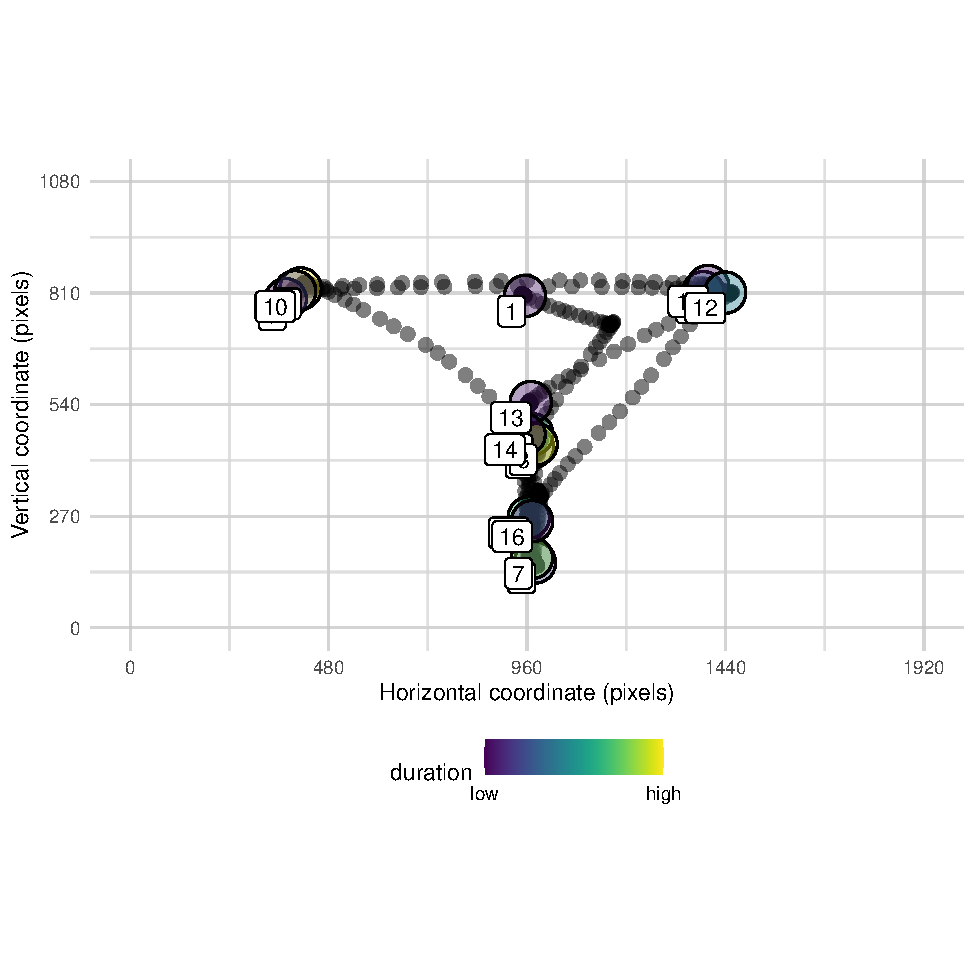
\includegraphics[keepaspectratio]{BRM_ms_files/figure-pdf/unnamed-chunk-15-1.pdf}}

}

\end{figure}%

In addition to eye data, a background image can be added to the plot,
which is useful for inspecting data over a representation of the
experimental task. If AOIs have been defined, these can be plotted as
well. Here we demonstrate the plotting of the saccades, AOIs, and a
background image:

\begin{Shaded}
\begin{Highlighting}[]
\FunctionTok{plot\_spatial}\NormalTok{(}\AttributeTok{sac\_data =}\NormalTok{ saccades,}
             \AttributeTok{AOIs =}\NormalTok{ HCL\_AOIs,}
             \AttributeTok{pID\_values =} \DecValTok{118}\NormalTok{,}
             \AttributeTok{trial\_values =} \DecValTok{6}\NormalTok{,}
             \AttributeTok{bg\_image =} \StringTok{"images/HCL\_sample\_image.png"}\NormalTok{)}
\end{Highlighting}
\end{Shaded}

\begin{figure}[H]

\caption{Saccades (blue arrows) and Area-Of-Interest regions (pink
shapes) for a single trial, against a background image.}

{\centering \pandocbounded{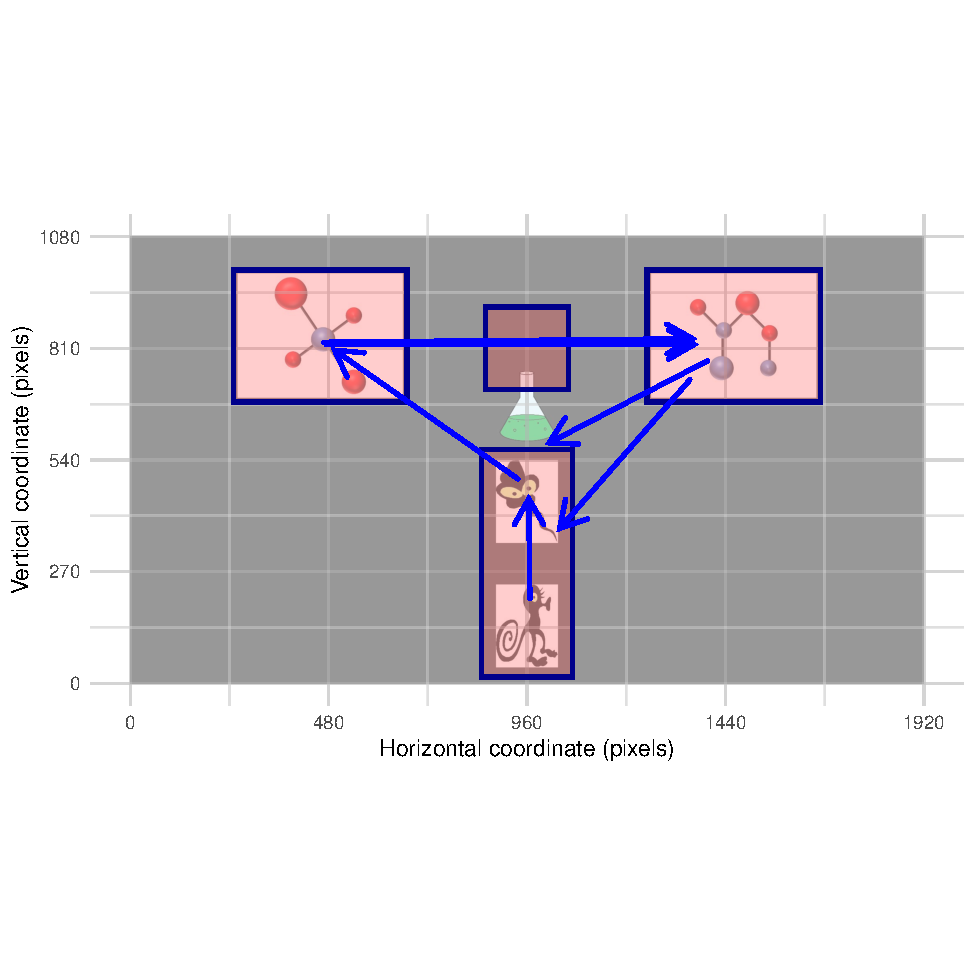
\includegraphics[keepaspectratio]{BRM_ms_files/figure-pdf/unnamed-chunk-16-1.pdf}}

}

\end{figure}%

The function \texttt{plot\_seq()} is useful for visualising data as a
series of plots, mapping out eye movements over the course of a single
trial. By default this function will plot a randomly selected trial from
the raw data that is passed to the function. Otherwise, specific trials
and participant values can be specified. The function requires a
``bin\_time'' parameter, that specifies the length of each time-period
within the trial. An optional parameter of ``bin\_range'' can be
specified to restrict the range of these periods that are presented. For
example here we plot data in periods of 1000 ms across the first four of
these periods.

\begin{Shaded}
\begin{Highlighting}[]
\FunctionTok{plot\_seq}\NormalTok{(}\AttributeTok{data =}\NormalTok{ data,}
         \AttributeTok{bin\_time =} \DecValTok{1000}\NormalTok{,}
         \AttributeTok{bin\_range =} \FunctionTok{c}\NormalTok{(}\DecValTok{1}\NormalTok{,}\DecValTok{4}\NormalTok{),}
         \AttributeTok{trial\_values =} \DecValTok{1}\NormalTok{,}
         \AttributeTok{pID\_values =} \DecValTok{118}\NormalTok{,}
         \AttributeTok{AOIs =}\NormalTok{ HCL\_AOIs,}
         \AttributeTok{bg\_image =} \StringTok{"images/HCL\_sample\_image.png"}\NormalTok{)}
\end{Highlighting}
\end{Shaded}

\begin{figure}[H]

\caption{The data from the same example trial, plotted across 4
consecutive bins of 1000 milliseconds}

{\centering \pandocbounded{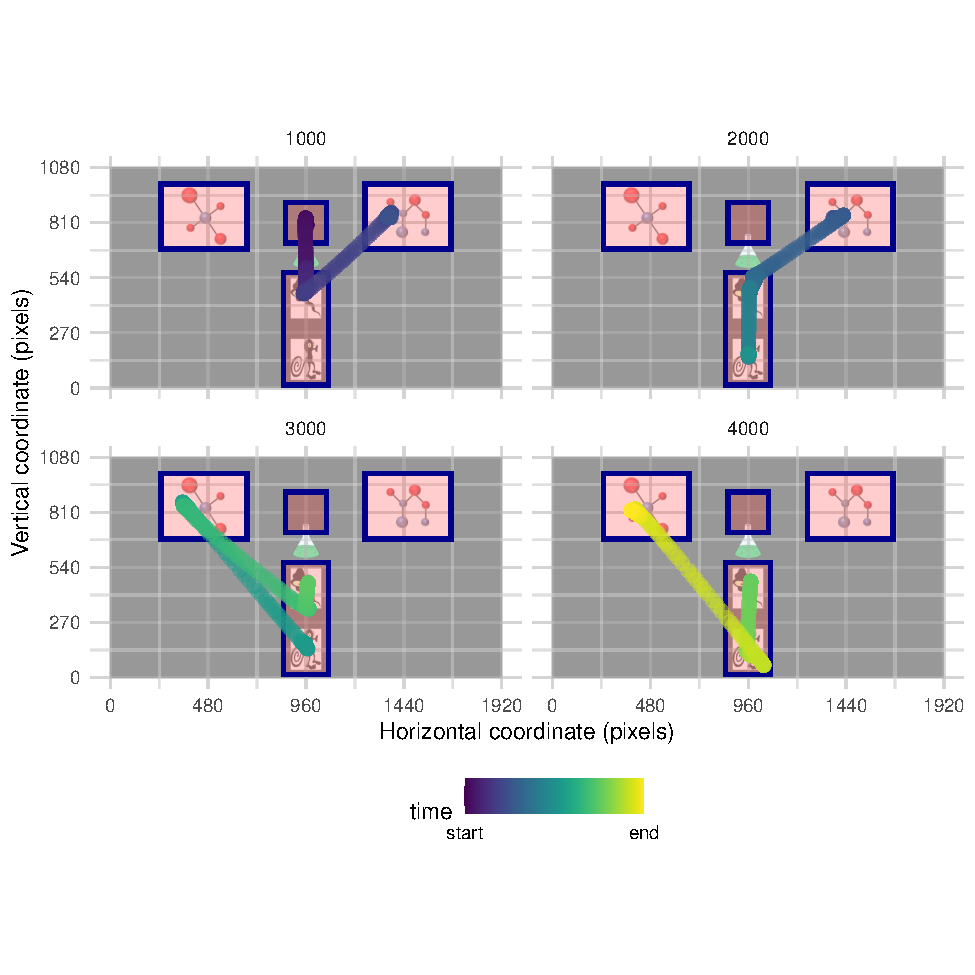
\includegraphics[keepaspectratio]{BRM_ms_files/figure-pdf/unnamed-chunk-17-1.pdf}}

}

\end{figure}%

The \texttt{plot\_AOI\_growth()} function offers a visualisation of the
progression of time spent on AOIs across a single trial. This can be
useful to see how participants interact with AOIs over time, and this
can be presented as either a plot of the cumulative time, or as a
proportion of the time spent in the trial.

\begin{Shaded}
\begin{Highlighting}[]
\CommentTok{\# plot absolute and then proportional}
\FunctionTok{plot\_AOI\_growth}\NormalTok{(}\AttributeTok{data =}\NormalTok{ data, }
                \AttributeTok{AOIs =}\NormalTok{ HCL\_AOIs, }
                \AttributeTok{type =} \StringTok{"abs"}\NormalTok{, }
                \AttributeTok{pID\_values =} \DecValTok{118}\NormalTok{,}
                \AttributeTok{trial\_values =} \DecValTok{1}\NormalTok{)}
\FunctionTok{plot\_AOI\_growth}\NormalTok{(}\AttributeTok{data =}\NormalTok{ data, }
                \AttributeTok{AOIs =}\NormalTok{ HCL\_AOIs, }
                \AttributeTok{type =} \StringTok{"prop"}\NormalTok{,  }
                \AttributeTok{pID\_values =} \DecValTok{118}\NormalTok{,}
                \AttributeTok{trial\_values =} \DecValTok{1}\NormalTok{)}
\end{Highlighting}
\end{Shaded}

\begin{figure}[H]

\caption{\label{fig-growth}Examples of the absolute and proportional
time plots from \texttt{plot\_AOI\_growth()}}

\begin{minipage}{0.50\linewidth}

\subcaption{\label{fig-abs}}

\centering{

\pandocbounded{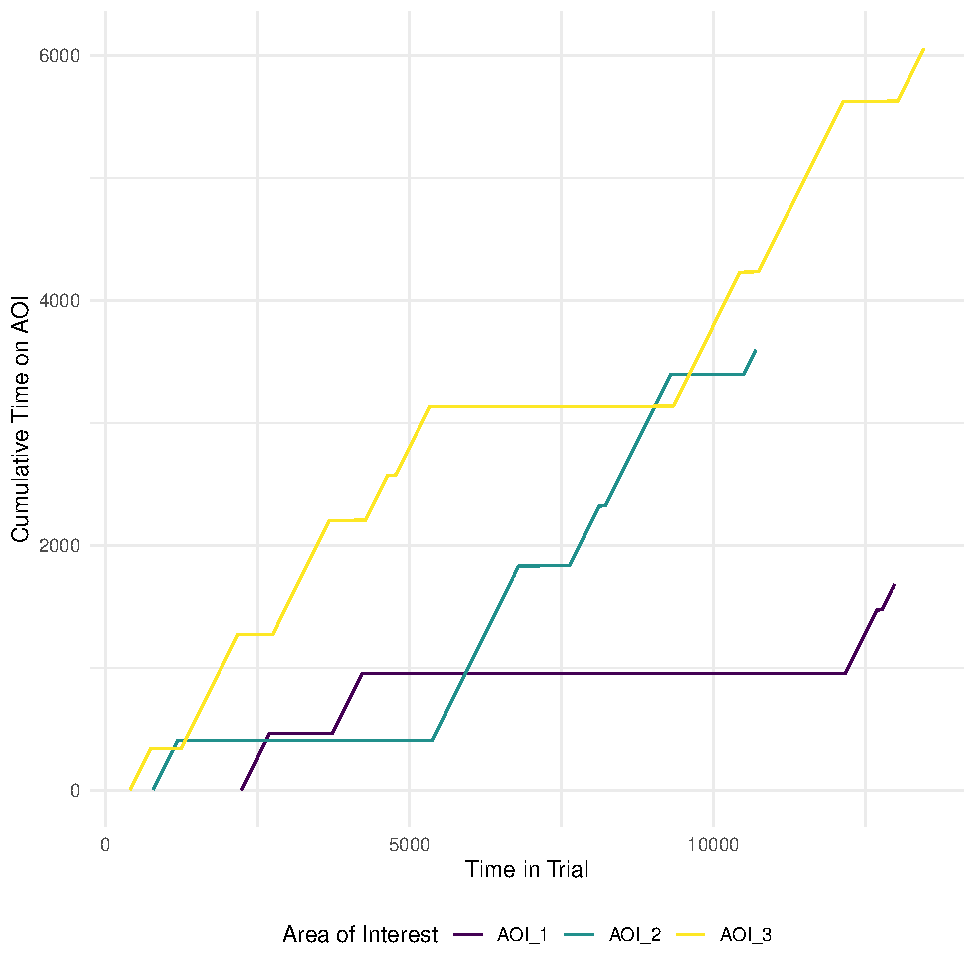
\includegraphics[keepaspectratio]{BRM_ms_files/figure-pdf/fig-abs-1.pdf}}

}

\end{minipage}%
%
\begin{minipage}{0.50\linewidth}

\subcaption{\label{fig-prop}}

\centering{

\pandocbounded{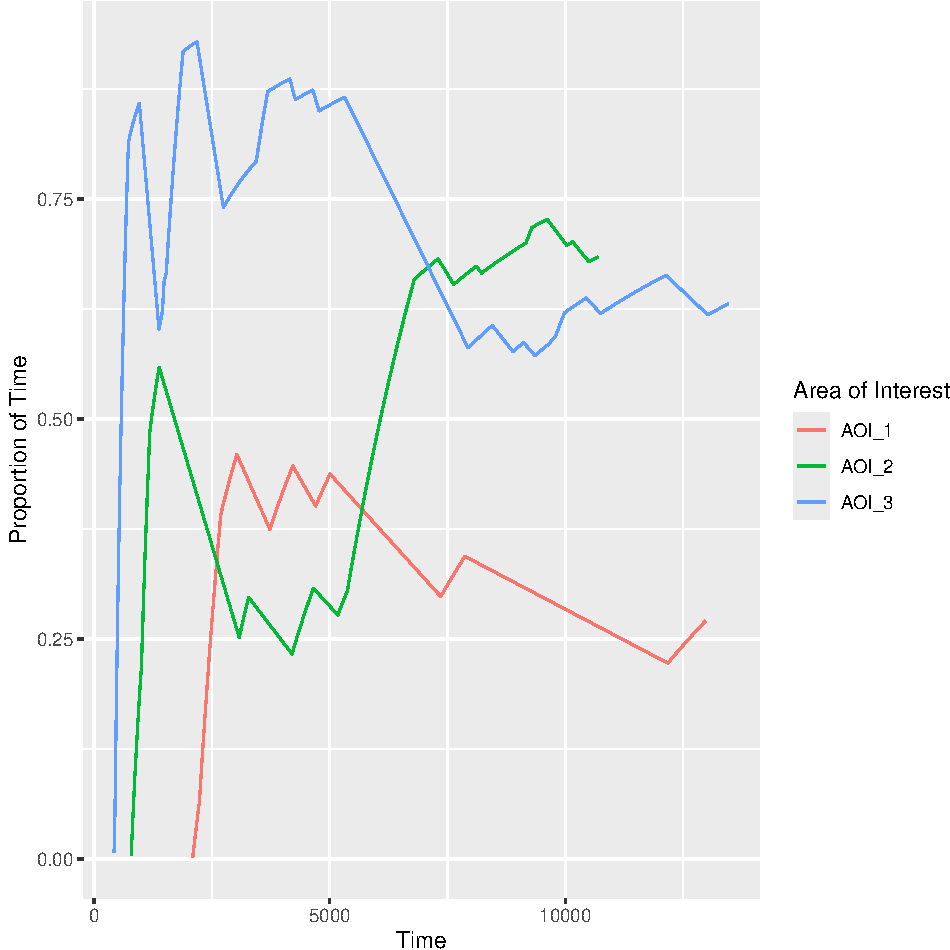
\includegraphics[keepaspectratio]{BRM_ms_files/figure-pdf/fig-prop-1.pdf}}

}

\end{minipage}%

\end{figure}%

A heatmap of eye gaze positions can be generated using
\texttt{plot\_heatmap()} which takes raw data as input. Like
\texttt{plot\_spatial()}, it is possible to select certain pID and
trial\_values, therefore offering a complementary visualisation of raw
data. As can be seen in Figure~\ref{fig-heatmap}, we can be reassured
that participants do indeed spend most of their time looking at the
stimuli on screen rather than in the empty space.
\texttt{plot\_heatmap()} also allows for the modification of the amount
of data displayed, using the \texttt{alpha\_range} parameter. This takes
a pair of values to specify a range between 0 and 1. The first value is
a cut off, controlling how much of the low frequency positions are not
displayed in the plot. The second value sets the transparancy of the
visible points.

\begin{Shaded}
\begin{Highlighting}[]
\FunctionTok{plot\_heatmap}\NormalTok{(data, }
             \AttributeTok{pID\_values =} \DecValTok{118}\NormalTok{,}
             \AttributeTok{trial\_values =} \FunctionTok{c}\NormalTok{(}\DecValTok{1}\NormalTok{,}\DecValTok{3}\NormalTok{),}
             \AttributeTok{alpha\_range =} \FunctionTok{c}\NormalTok{(}\FloatTok{0.1}\NormalTok{,}\DecValTok{1}\NormalTok{),}
             \AttributeTok{bg\_image =} \StringTok{"images/HCL\_sample\_image.png"}\NormalTok{)}
\end{Highlighting}
\end{Shaded}

\begin{figure}[H]

\caption{\label{fig-heatmap}A heatmap overlaid upon a sample stimuli
image demonstrating where the participants looked most over all trials}

\centering{

\pandocbounded{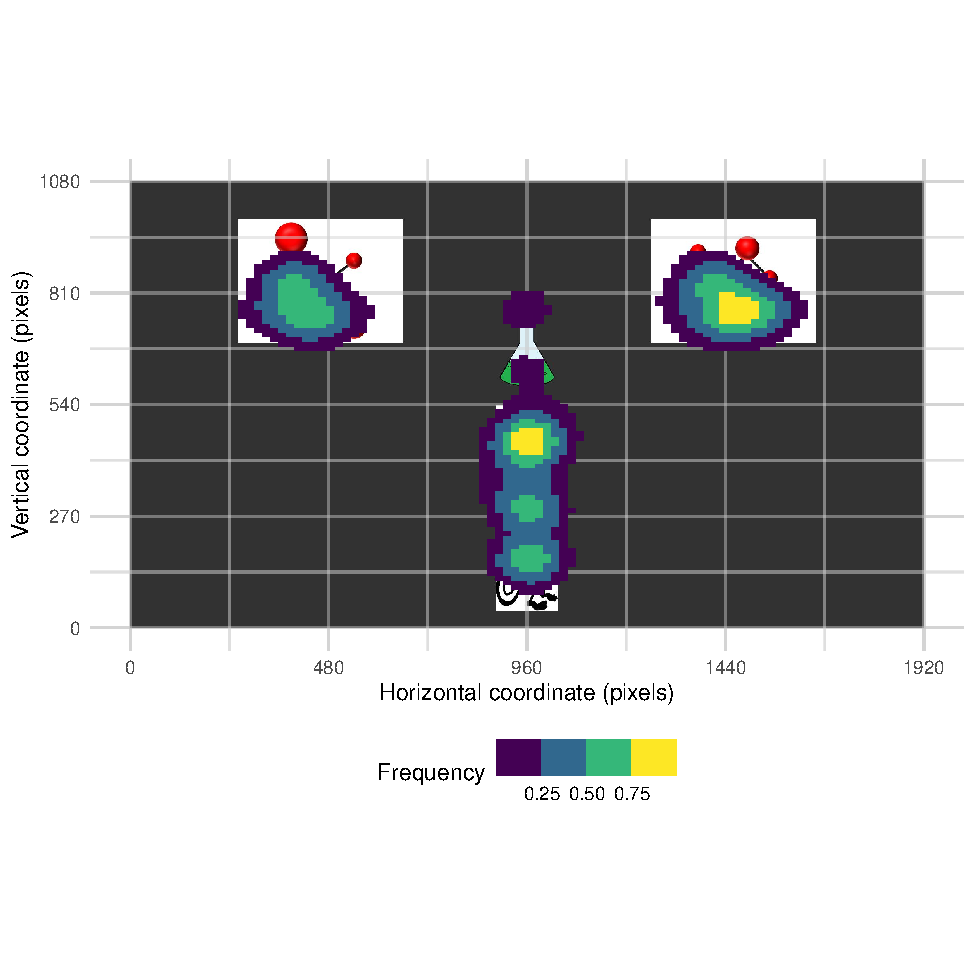
\includegraphics[keepaspectratio]{BRM_ms_files/figure-pdf/fig-heatmap-1.pdf}}

}

\end{figure}%

\subsection{Validation of fixation
metrics}\label{validation-of-fixation-metrics}

\emph{eyetools} uses implementations of common methods for extracting
fixations from raw data (\citeproc{ref-salvucci2000}{Salvucci \&
Goldberg, 2000}). To provide a simple validation of our primary fixation
algorithm, we took raw data collected independently from a researcher
outside of our lab on an unknown task. The researcher provided the raw
data and extracted fixations for a 6 minute period of data collection,
from Tobii Pro Lab software. From the raw data we used the
\emph{eyetools} \texttt{fixation\_dispersion()} and
\texttt{fixation\_VTI()} algorithms to compute fixations from randomly
drawn periods of 10 seconds. Figure~\ref{fig-tobii-comp} shows
side-by-side comparisons of Tobii and \emph{eyetools} extracted
fixations from 3 such periods (the raw data and analysis script for this
comparison is available in the manuscript repository for full
exploration of other periods). Somewhat unsurprisingly, the algorithms
show a very similar spread of fixations for these periods. Notably the
number of overall fixations differs across the samples, which is a
consequence of the particular parameters used to define fixations, such
as the dispersion tolerance and the minimum duration.

\begin{figure}[H]

\caption{\label{fig-tobii-comp}A comparison of extracted fixations from
Tobii Pro Lab (A:left), eyetools::fixation\_dispersion() (B:centre) and
eyetools::fixation\_VTI() (C:right), across 3 samples.}

\centering{

\pandocbounded{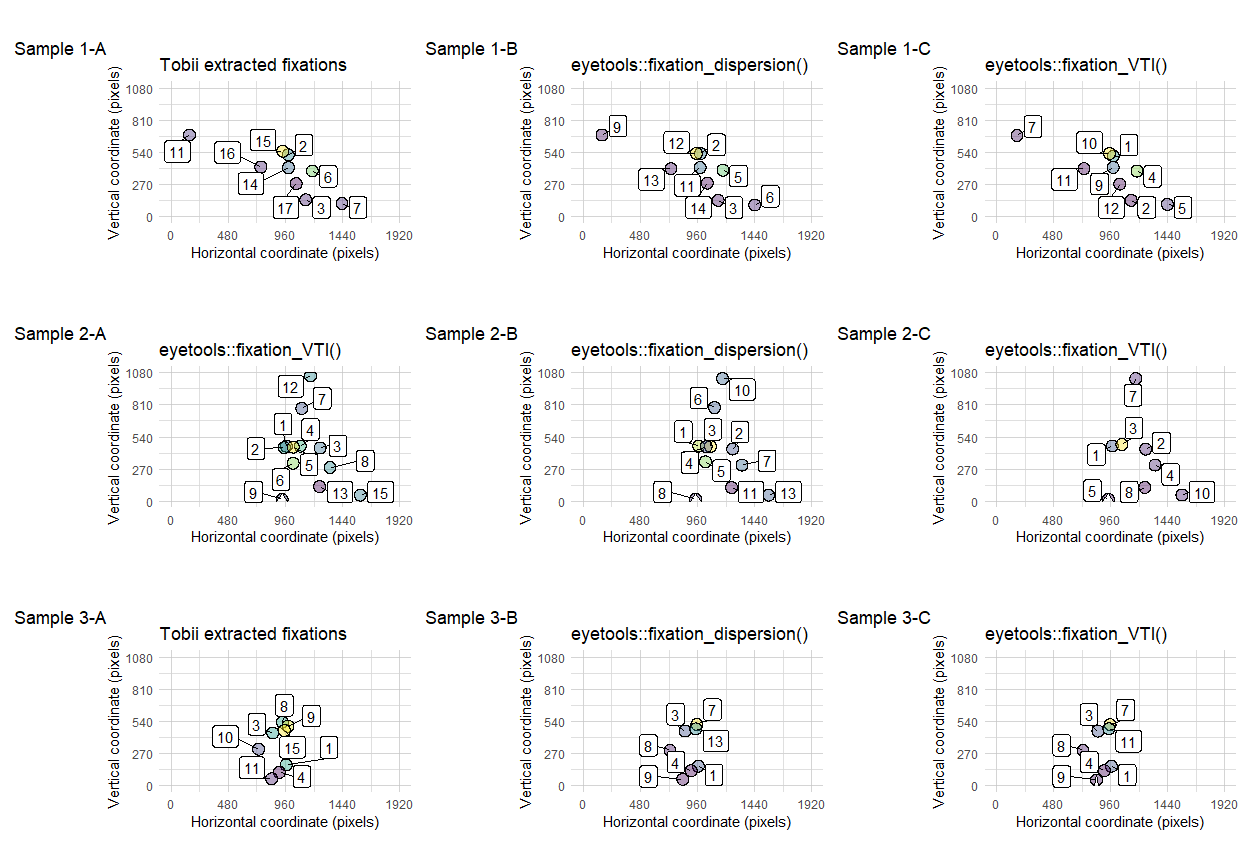
\includegraphics[keepaspectratio]{fixation_comparison.png}}

}

\end{figure}%

\subsection{Summary and future
directions}\label{summary-and-future-directions}

This paper has given an introduction and basic tutorial on working with
an open source R package for an analysis pipeline for eye data. We began
by identifying the current gaps in available tools for working with eye
data in reproducible pipelines. We then provided an overview of the
initial steps in working with raw eye data and the conversion of raw eye
data into a usable format for working with the functions in
\emph{eyetools}. We then covered many useful steps in the analysis
pipeline using functions available in the \emph{eyetools} package that
included the repairing and normalising of the data, the detection of
events such as fixations and saccades, and the trial level analysis of
data patterns, such as time on areas of interest, and the sequencing of
entries to areas of interest.

This tutorial offers a step-by-step walk-through for handling eye data
using R, demonstrating that the \emph{eyetools} package provides a set
of tools that will lead to reproducible analysis steps for many
experimental psychologists. It is hopefully clear that the functions in
\emph{eyetools} are flexible and powerful, yet ultimately simple to
implement. While these functions represent some initial steps in eye
data analysis, since the objects that result from these functions are
standard formats in R (i.e., dataframes and plots), they will provide
the user a means to enable more complex or nuanced analyses.

\emph{eyetools} offers an open-source toolset that holds no hidden nor
proprietary functionality. The major benefits of open-source tools are
extensive: not only do they allow for full inspection and
reproducibility of analyses, but they also support and enable the
development and sharing of new analysis functions. There are a number of
obvious features that would be hugely beneficial in future versions of
\emph{eyetools}. For example, while the package provides means to
determine the order of eye-movements (\texttt{AOI\_seq()}) there is no
means to compare these patterns across different trials or periods. Such
``scan-path analyses'' have been used effectively in cognitive studies
and so algorithms to conduct these analyses would be an obvious next
step. There are also no functions within the package to handle
pupilometry data, despite the obvious benefits of analysing these data.
From a development perspective, while these features would be hugely
beneficial to the package, they will only be implemented as and when
there is a need in our research. Thus our hope for \emph{eyetools} is
that future versions will benefit from user engagement and an expansion
of the toolset to enable an ever more powerful set of features. We
believe eyetools provides a solid foundation for this collaborative
venture.

\subsection{Data and code
availability}\label{data-and-code-availability}

This manuscript was written in Quarto and can be reproduced from the
manuscript source files which are available at
\url{https://github.com/tombeesley/BRM_eyetools} . The manuscript
details functions from the latest development version of \emph{eyetools}
which is 0.9.3. We welcome contributions to the development of
\emph{eyetools} by posting bug reports and suggested improvements at
\url{https://github.com/tombeesley/eyetools/issues} .

\subsection{Declarations}\label{declarations}

\subsubsection{Funding}\label{funding}

Not applicable

\subsubsection{Conflicts of interest/Competing
interests}\label{conflicts-of-interestcompeting-interests}

Not applicable

\subsubsection{Ethics approval}\label{ethics-approval}

Not applicable

\subsubsection{Consent to participate}\label{consent-to-participate}

Not applicable

\subsubsection{Consent for publication}\label{consent-for-publication}

Not applicable

\subsubsection{Availability of data and
materials}\label{availability-of-data-and-materials}

This manuscript was written in Quarto and can be reproduced from the
manuscript source files which are available at
\url{https://github.com/tombeesley/BRM_eyetools}

\subsubsection{Code availability}\label{code-availability}

The manuscript details functions from the latest CRAN version of
\emph{eyetools} which is 0.9.2. The package source code is available at
\url{https://github.com/tombeesley/eyetools}

\subsubsection{Authors' contributions}\label{authors-contributions}

TB - project inception; software design and coding; primary author of
the manuscript. MI - software design and coding; secondary author of the
manuscript

\subsection{References}\label{references}

\phantomsection\label{refs}
\begin{CSLReferences}{1}{0}
\bibitem[\citeproctext]{ref-beesley2015}
Beesley, T., Nguyen, K. P., Pearson, D., \& Le Pelley, M. E. (2015).
Uncertainty and predictiveness determine attention to cues during human
associative learning. \emph{Quarterly Journal of Experimental
Psychology}, \emph{68}(11), 2175--2199.
\url{https://doi.org/10.1080/17470218.2015.1009919}

\bibitem[\citeproctext]{ref-beesley2019}
Beesley, T., Pearson, D., \& Le Pelley, M. (2019). \emph{Chapter 1 - eye
tracking as a tool for examining cognitive processes} (G. Foster, Ed.;
pp. 1--30). Academic Press.
\url{https://doi.org/10.1016/B978-0-12-813092-6.00002-2}

\bibitem[\citeproctext]{ref-vanduren1995}
Duren, L. L. van, \& Sanders, A. F. (1995). Signal processing during and
across saccades. \emph{Acta Psychologica}, \emph{89}(2), 121--147.
\url{https://doi.org/10.1016/0001-6918(94)00029-G}

\bibitem[\citeproctext]{ref-irwin1995}
Irwin, D. E., Carlson-Radvansky, L. A., \& Andrews, R. V. (1995).
Information processing during saccadic eye movements. \emph{Acta
Psychologica}, \emph{90}(1), 261--273.
\url{https://doi.org/10.1016/0001-6918(95)00024-O}

\bibitem[\citeproctext]{ref-salvucci2000}
Salvucci, D. D., \& Goldberg, J. H. (2000). \emph{the symposium}.
71--78. \url{https://doi.org/10.1145/355017.355028}

\bibitem[\citeproctext]{ref-sanders1985}
Sanders, A. F., \& Houtmans, M. J. M. (1985). There is no central
stimulus encoding during saccadic eye shifts: A case against general
parallel processing notions. \emph{Acta Psychologica}, \emph{60}(2),
323--338. \url{https://doi.org/10.1016/0001-6918(85)90060-5}

\end{CSLReferences}






\end{document}
